\documentclass{beamer}
%
% Choose how your presentation looks.
%
% For more themes, color themes and font themes, see:
% http://deic.uab.es/~iblanes/beamer_gallery/index_by_theme.html
%
\mode<presentation>
{
  \usetheme{default}      % or try Darmstadt, Madrid, Warsaw, ...
  \usecolortheme{default} % or try albatross, beaver, crane, ...
  \usefonttheme{default}  % or try serif, structurebold, ...
  \setbeamertemplate{navigation symbols}{}
  \setbeamertemplate{caption}[numbered]
} 

\usepackage[english]{babel}
\usepackage[utf8x]{inputenc}

\title[Course presentation]{Introduction to machine learning}
\author{Alexis Zubiolo}
\institute{Adcash Bulgaria}
\date{September 15, 2016}

\begin{document}

\begin{frame}
  \titlepage
\end{frame}

% Uncomment these lines for an automatically generated outline.
%\begin{frame}{Outline}
%  \tableofcontents
%\end{frame}

\begin{frame}
\vfill
\textbf{Disclamer}: This presentation is a promotion of the \textit{Introduction to machine learning} course I will be giving at IT STEP.
\vfill
\end{frame}

\begin{frame}{Presentation outline}

\vfill
\begin{itemize}
  \item Introduction: What is machine learning?
\vfill
  \item A few practical examples
  \begin{itemize}
  	\item classification
  	\item regression
  \end{itemize}
\vfill
  \item Goals and presentation of the course 
\vfill
  \item Questions and answers
\end{itemize}
\vfill

\end{frame}

\begin{frame}{What is machine learning?}
\vfill
Let's start with a simple example\ldots
\vfill
\begin{figure}
\centering
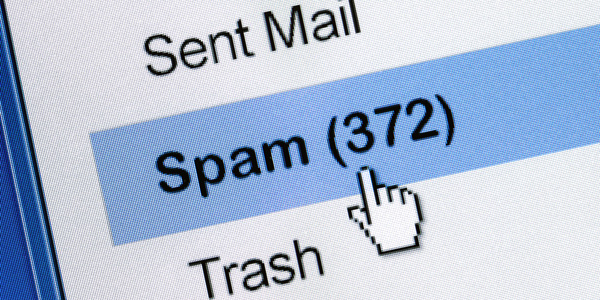
\includegraphics[width=\textwidth]{images/spam.jpg}
\end{figure}
\vfill
How to filter spam emails \textbf{automatically}?
\vfill
\end{frame}

\begin{frame}{Machine learning paradigm}
~\\
\vfill
Goal: Build algorithms that can 
\begin{itemize}
	\item \textbf{learn} from data
	\item \textbf{make predictions} on data
\end{itemize}
\vfill
\begin{figure}
\centering
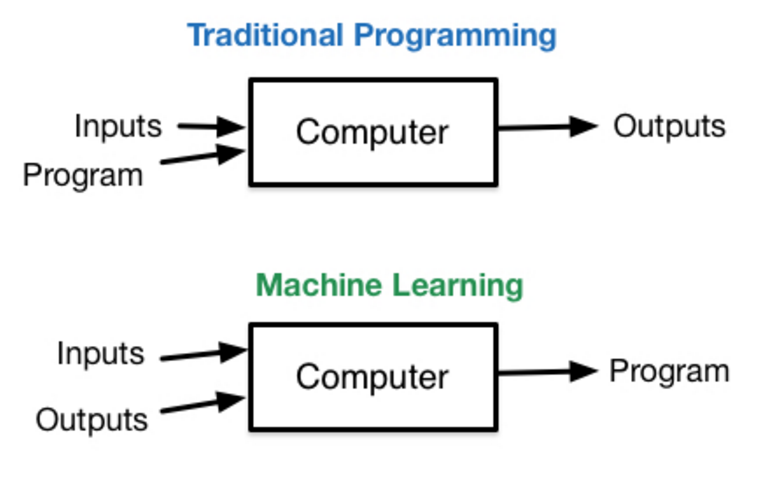
\includegraphics[width=\textwidth]{images/ml_vs_traditional.png}
\end{figure}
\vfill
\end{frame}

\begin{frame}{Main components of machine learning}

\vfill
Mathematics
\begin{itemize}
	\item Linear algebra
	\item Calculus
	\item Numerical optimization
\end{itemize}
\vfill
Statistics, probability theory
\vfill
Computer science
\vfill

\end{frame}

\begin{frame}{Example 1: Regression}

Regression = output is a \textbf{continuous} numerical value
\vfill
Example: \textbf{Estimate the price} of an apartment
\begin{itemize}
	\item input: \textbf{information} about the apartment
	\item output: \textbf{price}
\end{itemize}
\vfill
\pause
\begin{table}
\centering
\begin{tabular}{r|r}
living area (m$^2$) & price (1000's euros) \\\hline
50 & 30 \\
76 & 48 \\
26 & 12 \\
102 & 90 \\
\pause
61 & ?
\end{tabular}
\end{table}
\vfill
Linear model: price = \textbf{a} $\times$ area + \textbf{b}
\vfill
Problem: optimal values for \textbf{a} and \textbf{b}?

\end{frame}

\begin{frame}{Regression}

More data for a richer model:
\vfill
\begin{table}
\centering
\begin{tabular}{r|r|r}
living area (m$^2$) &  \textbf{\# bedrooms} & price (1000's euros) \\\hline
50 & \textbf{1} & 30\\
76 & \textbf{2} & 48\\
26 & \textbf{1} & 12\\
102 & \textbf{3} & 90\\
61 & \textbf{2} & ?
\end{tabular}
\end{table}

\vfill
Linear model: price = \textbf{a} $\times$ area + \textbf{b} $\times$ \# bedrooms + \textbf{c}
\vfill
Problem: optimal values for \textbf{a}, \textbf{b} and \textbf{c}?
\end{frame}

\begin{frame}{Example 2: Classification}
\vfill
Classification = output is a \textbf{label}
\vfill
Examples: 
\pause
\vfill
\begin{itemize}
	\item Spam filtering
	\begin{itemize}
		\item input: email (text, subject, address, \ldots)
		\item output: \textbf{spam} or \textbf{not spam}
	\end{itemize}
\pause
\vfill
	\item Object recognition in images or videos
	\begin{itemize}
		\item input: image or video
		\item (example) output: \textbf{face} or \textbf{not a face}
	\end{itemize}
\pause
\vfill
	\item Image classification/description
	\begin{itemize}
		\item input: image
		\item output: image \textbf{description} or \textbf{label} (apple, car, \ldots)
	\end{itemize}
\end{itemize}
\vfill

\end{frame}

\begin{frame}{Automated image description generation}

\begin{figure}
\centering
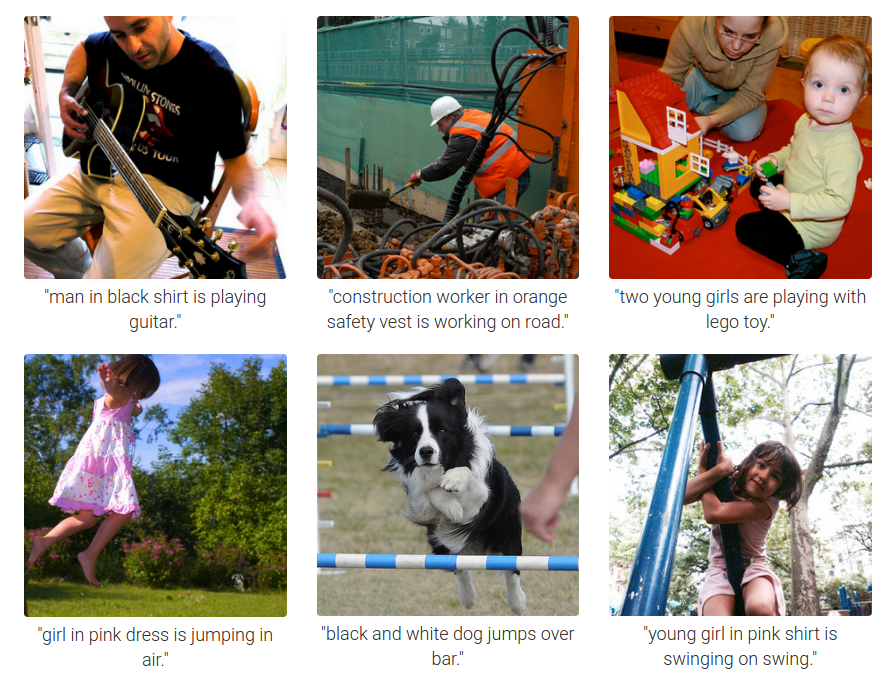
\includegraphics[width=\textwidth]{images/generated_descriptions.png}
\end{figure}
\end{frame}

\begin{frame}{Automated image description generation}

\begin{figure}
\vspace*{-0.15cm}
\centering
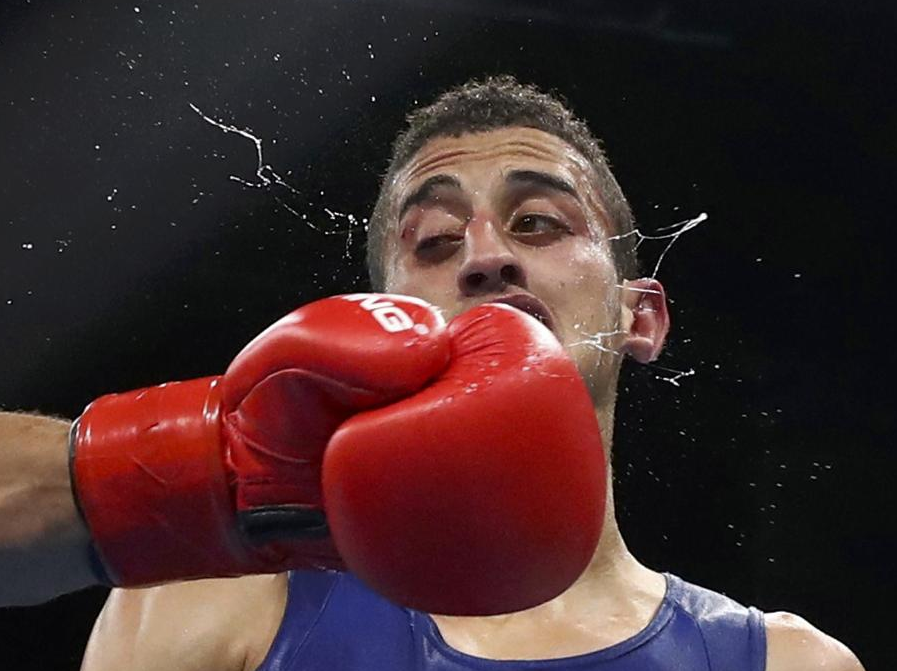
\includegraphics[width=\textwidth]{images/boxing.png}\\
\pause
A man holding a red apple in his mouth
\end{figure}

\end{frame}

\begin{frame}{Other topics}
\vfill
Machine learning is a wide and growing field. It also includes:	
\pause 
\vfill
\begin{itemize}
	\item Clustering (no predifined label/output)
\pause 
\vfill
	\item Dimensionality reduction
\pause 
\vfill
	\item \ldots
\end{itemize}
\vfill
\end{frame}

\begin{frame}{The course}

Important note: This is an \textbf{introduction} course. 
\vfill
\pause 
Goals:
\begin{itemize}
	\item Introduce \textbf{main concepts} of machine learning
	\item \textbf{Implement} these concepts in Python (Scikit-learn)
\end{itemize}
\vfill
\pause 
Practical information:
\begin{itemize}
	\item $\sim$ \textbf{10 sessions}, 1 per week (early October -- mid December)
	\item $\sim$ \textbf{90min} sessions
	\item Thursdays at $\sim$ 6:30pm
	\item Alternating between \textbf{lectures and lab sessions}
\end{itemize}
\end{frame}

\begin{frame}
\vfill
\centering
\huge{Thank you! Questions?}
\vfill
\end{frame}

\end{document}
